% !TEX encoding = UTF-8 Unicode
%%%%%%%%%%%%%%%%%%%%%%%%%%%%%%%%%%%%%%%%%
% Beamer Presentation
% LaTeX Template
% Version 1.0 (10/11/12)
%
% This template has been downloaded from:
% http://www.LaTeXTemplates.com
%
% License:
% CC BY-NC-SA 3.0 (http://creativecommons.org/licenses/by-nc-sa/3.0/)
%
%%%%%%%%%%%%%%%%%%%%%%%%%%%%%%%%%%%%%%%%%

%----------------------------------------------------------------------------------------
%	PACKAGES AND THEMES
%----------------------------------------------------------------------------------------

\documentclass{beamer}

\mode<presentation> {

% The Beamer class comes with a number of default slide themes
% which change the colors and layouts of slides. Below this is a list
% of all the themes, uncomment each in turn to see what they look like.

%\usetheme{default}
%\usetheme{AnnArbor}
%\usetheme{Antibes}
%\usetheme{Bergen}
%\usetheme{Berkeley}
%\usetheme{Berlin}
%\usetheme{Boadilla}
%\usetheme{CambridgeUS}
%\usetheme{Copenhagen}
%\usetheme{Darmstadt}
%\usetheme{Dresden}
%\usetheme{Frankfurt}
%\usetheme{Goettingen}
%\usetheme{Hannover}
%\usetheme{Ilmenau}
%\usetheme{JuanLesPins}
%\usetheme{Luebeck}
\usetheme{Madrid}
%\usetheme{Malmoe}
%\usetheme{Marburg}
%\usetheme{Montpellier}
%\usetheme{PaloAlto}
%\usetheme{Pittsburgh}
%\usetheme{Rochester}
%\usetheme{Singapore}
%\usetheme{Szeged}
%\usetheme{Warsaw}

% As well as themes, the Beamer class has a number of color themes
% for any slide theme. Uncomment each of these in turn to see how it
% changes the colors of your current slide theme.

%\usecolortheme{albatross}
%\usecolortheme{beaver}
%\usecolortheme{beetle}
%\usecolortheme{crane}
%\usecolortheme{dolphin}
%\usecolortheme{dove}
%\usecolortheme{fly}
%\usecolortheme{lily}
%\usecolortheme{orchid}
%\usecolortheme{rose}
%\usecolortheme{seagull}
%\usecolortheme{seahorse}
%\usecolortheme{whale}
%\usecolortheme{wolverine}

%\setbeamertemplate{footline} % To remove the footer line in all slides uncomment this line
%\setbeamertemplate{footline}[page number] % To replace the footer line in all slides with a simple slide count uncomment this line

%\setbeamertemplate{navigation symbols}{} % To remove the navigation symbols from the bottom of all slides uncomment this line
}

\usepackage{graphicx} % Allows including images
\usepackage{booktabs} % Allows the use of \toprule, \midrule and \bottomrule in tables
\usepackage{xeCJK}
\usepackage{color}
\usepackage{listings}
\lstset{numbers=left}
\usepackage{tikz}


%----------------------------------------------------------------------------------------
%	TITLE PAGE
%----------------------------------------------------------------------------------------

\title[Sockets]{Sockets} % The short title appears at the bottom of every slide, the full title is only on the title page

\author{张海宁} % Your name
\institute[计算机科学与技术学院] % Your institution as it will appear on the bottom of every slide, may be shorthand to save space
{
贵州大学 \\ % Your institution for the title page
\medskip
\textit{hnzhang1@gzu.edu.cn} % Your email address
}
\date{\today} % Date, can be changed to a custom date

\begin{document}

\begin{frame}
\titlepage % Print the title page as the first slide
\end{frame}

\begin{frame}
\frametitle{Overview} % Table of contents slide, comment this block out to remove it
\tableofcontents % Throughout your presentation, if you choose to use \section{} and \subsection{} commands, these will automatically be printed on this slide as an overview of your presentation
\end{frame}

%----------------------------------------------------------------------------------------
%	PRESENTATION SLIDES
%----------------------------------------------------------------------------------------
\section{Sockets}
\begin{frame}
\Huge{\centerline{Sockets}}
\end{frame}
\subsection{What is a Socket}
\begin{frame}
\Huge{\centerline{What is a Socket}}
\end{frame}
\begin{frame}{Socket}
Socket是一种进程间的通信机制。
\begin{block}{进程间通信}
\center{
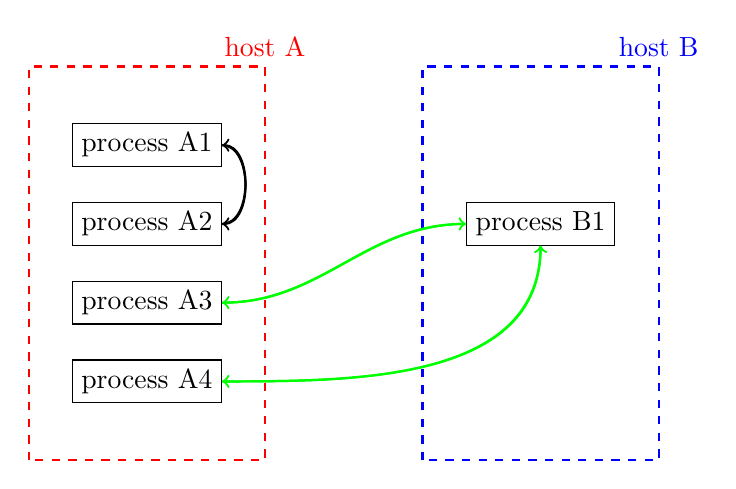
\begin{tikzpicture}
\draw [thick,red,dashed,above] (0,0) rectangle (3,5) node{host A};
\node [draw,rectangle] (pa1) at(1.5,4){process A1};
\node [draw,rectangle] (pa2) at(1.5,3){process A2};
\node [draw,rectangle] (pa3) at(1.5,2){process A3};
\node [draw,rectangle] (pa4) at(1.5,1){process A4};
\draw [thick,blue,dashed,above] (5,0) rectangle (8,5)node{host B};
\node [draw,rectangle] (pb1) at(6.5,3){process B1};
%\node [draw,rectangle] (pb2) at(6.5,2){...};
\draw[thick,->](pa1) to[out=0,in=360] (pa2);
\draw[thick,->](pa2) to[out=0,in=360] (pa1);
\draw[thick,->,green](pa3) to[out=0,in=180] (pb1);
\draw[thick,->,green](pa4) to[out=0,in=270] (pb1);
\draw[thick,->,green](pb1) to[out=180,in=360] (pa3);
\draw[thick,->,green](pb1) to[out=270,in=360] (pa4);
\end{tikzpicture}
}
\end{block}
\end{frame}

\begin{frame}{Socket通信过程 I}
服务器端的进程process B通过socket系统调用创建了一个socket, 这个socket对外表现就是一个端口。比如web常用端口80 。
该socket随即调用accept方法,等待客户端的连接。
%\begin{block}{Socket通信过程}
\center{
\begin{tikzpicture}
\draw [thick,red,dashed,above] (0,0) rectangle (3,5) node{Client};

%\node [draw,rectangle] (pa3) at(1.5,2){process A3};
%\node [draw,rectangle] (pa4) at(1.5,1){process A4};
\draw [thick,blue,dashed,above] (6,0) rectangle (9,5)node{Server};
\node [draw,rectangle] (pb1) at(7.5,3){process B};
\node [draw,rectangle,left] (ss) at(pb1.west) {socket};
\node [draw,rectangle] (act) at (5.8,4){accept};
\draw [->,thick] (ss) to[out=90,in=270] (act);
%\draw[thick,->](pa1) to[out=0,in=360] (pa2);
%\draw[thick,->](pa2) to[out=0,in=360] (pa1);
%\draw[thick,->,green](pa3) to[out=0,in=180] (pb1);
%\draw[thick,->,green](pa4) to[out=0,in=270] (pb1);
%\draw[thick,->,green](pb1) to[out=180,in=360] (pa3);
%\draw[thick,->,green](pb1) to[out=270,in=360] (pa4);
\end{tikzpicture}
}
%\end{block}
\end{frame}
\begin{frame}{Socket通信过程 II}
客户端的进程process A通过socket系统调用创建一个socket。
%\begin{block}{Socket通信过程}
\center{
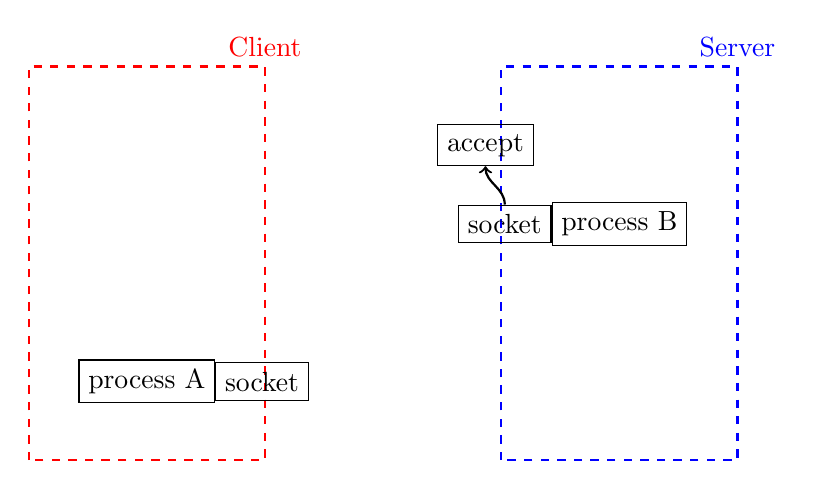
\begin{tikzpicture}
\draw [thick,red,dashed,above] (0,0) rectangle (3,5) node{Client};

%\node [draw,rectangle] (pa3) at(1.5,2){process A3};
\node [draw,rectangle] (pa1) at(1.5,1){process A};
\node [draw,rectangle,right] (cs) at(pa1.east) {socket};

\draw [thick,blue,dashed,above] (6,0) rectangle (9,5)node{Server};
\node [draw,rectangle] (pb1) at(7.5,3){process B};
\node [draw,rectangle,left] (ss) at(pb1.west) {socket};
\node [draw,rectangle] (act) at (5.8,4){accept};
\draw [->,thick] (ss) to[out=90,in=270] (act);
%\draw[thick,->](pa1) to[out=0,in=360] (pa2);
%\draw[thick,->](pa2) to[out=0,in=360] (pa1);
%\draw[thick,->,green](pa3) to[out=0,in=180] (pb1);
%\draw[thick,->,green](pa4) to[out=0,in=270] (pb1);
%\draw[thick,->,green](pb1) to[out=180,in=360] (pa3);
%\draw[thick,->,green](pb1) to[out=270,in=360] (pa4);
\end{tikzpicture}
}
%\end{block}
\end{frame}

\begin{frame}{Socket通信过程 III}
客户端的进程process A创建的socket将服务器的地址和端口传递给connect方法。
%\begin{block}{Socket通信过程}
\center{
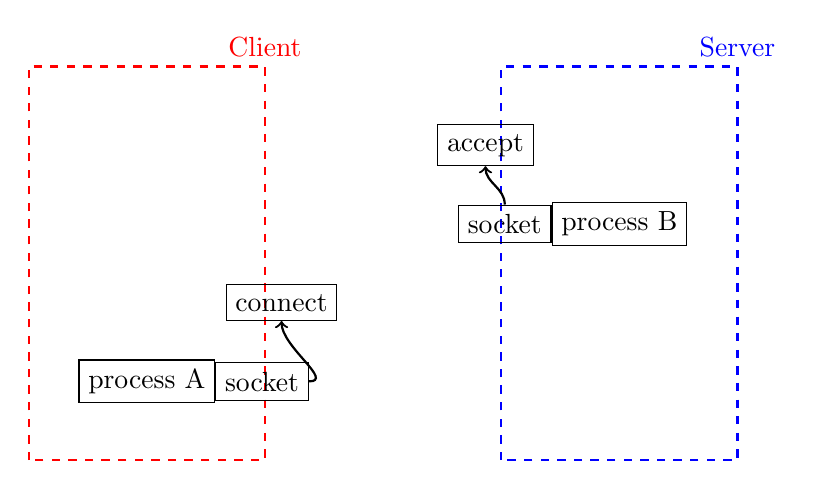
\begin{tikzpicture}
\draw [thick,red,dashed,above] (0,0) rectangle (3,5) node{Client};

%\node [draw,rectangle] (pa3) at(1.5,2){process A3};
\node [draw,rectangle] (pa1) at(1.5,1){process A};
\node [draw,rectangle,right] (cs) at(pa1.east) {socket};
\node [draw,rectangle,right] (conn) at(2.5,2) {connect};
\draw [->,thick] (cs) to[out=0,in=270] (conn);

\draw [thick,blue,dashed,above] (6,0) rectangle (9,5)node{Server};
\node [draw,rectangle] (pb1) at(7.5,3){process B};
\node [draw,rectangle,left] (ss) at(pb1.west) {socket};
\node [draw,rectangle] (act) at (5.8,4){accept};
\draw [->,thick] (ss) to[out=90,in=270] (act);
%\draw[thick,->](pa1) to[out=0,in=360] (pa2);
%\draw[thick,->](pa2) to[out=0,in=360] (pa1);
%\draw[thick,->,green](pa3) to[out=0,in=180] (pb1);
%\draw[thick,->,green](pa4) to[out=0,in=270] (pb1);
%\draw[thick,->,green](pb1) to[out=180,in=360] (pa3);
%\draw[thick,->,green](pb1) to[out=270,in=360] (pa4);
\end{tikzpicture}
}
%\end{block}
\end{frame}

\begin{frame}{Socket通信过程 IV}
客户端与服务端建立连接。然后processA 和B就像操作文件描述符一样可以对socket进行操作了。
%\begin{block}{Socket通信过程}
\center{
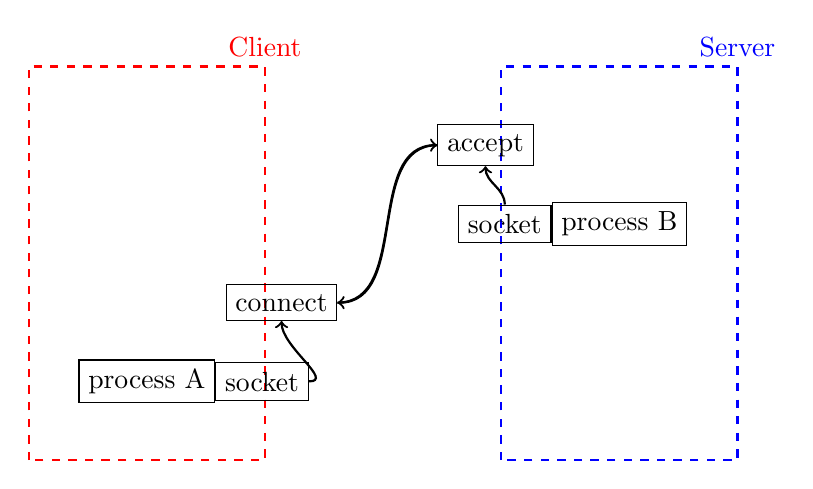
\begin{tikzpicture}
\draw [thick,red,dashed,above] (0,0) rectangle (3,5) node{Client};

%\node [draw,rectangle] (pa3) at(1.5,2){process A3};
\node [draw,rectangle] (pa1) at(1.5,1){process A};
\node [draw,rectangle,right] (cs) at(pa1.east) {socket};
\node [draw,rectangle,right] (conn) at(2.5,2) {connect};
\draw [->,thick] (cs) to[out=0,in=270] (conn);

\draw [thick,blue,dashed,above] (6,0) rectangle (9,5)node{Server};
\node [draw,rectangle] (pb1) at(7.5,3){process B};
\node [draw,rectangle,left] (ss) at(pb1.west) {socket};
\node [draw,rectangle] (act) at (5.8,4){accept};
\draw [->,thick] (ss) to[out=90,in=270] (act);

\draw[->,thick] (conn) to[out=0,in=180] (act);
\draw[->,thick] (act) to[out=180,in=360] (conn);
%\draw[thick,->](pa1) to[out=0,in=360] (pa2);
%\draw[thick,->](pa2) to[out=0,in=360] (pa1);
%\draw[thick,->,green](pa3) to[out=0,in=180] (pb1);
%\draw[thick,->,green](pa4) to[out=0,in=270] (pb1);
%\draw[thick,->,green](pb1) to[out=180,in=360] (pa3);
%\draw[thick,->,green](pb1) to[out=270,in=360] (pa4);
\end{tikzpicture}
}
%\end{block}
\end{frame}

%-----------------------------------------------
\section{Create a Socket}
\begin{frame}
\Huge{\centerline{Create a Socket}}
\end{frame}
\begin{frame}[fragile]{socket系统调用}
socket() creates an endpoint for communication and returns a descriptor.
\begin{block}{原型}
\begin{verbatim}
     #include <sys/socket.h>

     int
     socket(int domain, int type, int protocol);
\end{verbatim}
\end{block}
\end{frame}
\begin{frame}{socket-domain}
     The domain parameter specifies a communications domain within which communication will take place; this selects the protocol family which should be used.  These families are defined in
     the include file <sys/socket.h>.  The domains are as table \ref{skt-dm}.
\begin{table}
\begin{tabular}{ll}
\toprule
\textbf{Domain}&\textbf{Description}\\
\midrule
           \textcolor{red}{PF\_LOCAL}    &    Host-internal protocols, formerly called PF\_UNIX\\
           PF\_UNIX    &     Host-internal protocols, deprecated, use PF\_LOCAL\\
           \textcolor{red}{PF\_INET}       &  Internet version 4 protocols\\
           PF\_ROUTE   &     Internal Routing protocol\\
           PF\_KEY         & Internal key-management function\\
           PF\_INET6       & Internet version 6 protocols\\
           PF\_SYSTEM    &   System domain\\
           PF\_NDRV        & Raw access to network device\\
           \bottomrule
           \end{tabular}
\caption{Domain of socket}
\label{skt-dm}
\end{table}

\end{frame}
\begin{frame}{socket-type}
     The socket has the indicated type, which specifies the semantics of communication.  Currently defined types are:
\begin{enumerate}
\item
           SOCK\_STREAM
        \item   SOCK\_DGRAM
          \item SOCK\_RAW
\end{enumerate}
     A SOCK\_STREAM type provides sequenced, reliable, two-way connection based byte streams.  An out-of-band data(like urgent mode in tcp) transmission mechanism may be supported.  
     
     A SOCK\_DGRAM socket supports datagrams (connectionless, unreliable messages of a fixed (typically small) maximum length). 
     
      SOCK\_RAW sockets provide access to internal network protocols and interfaces.  The type
     SOCK\_RAW, which is available only to the super-user.
\end{frame}
\begin{frame}{socket-protocol}
The protocol used for communication is usually determined by the socket type and domain. There is normally no choice. The protocol parameter is used where there is a choice. \textcolor{red}{0 }selects the default protocol, which is used in all the examples in our course.
\end{frame}
\begin{frame}{Name a socket}
To make a socket (as created by a call to socket) available for use by other processes, a server program needs to give the socket a name. 

Thus, PF\_LOCAL sockets are associated with a file system pathname. 

PF\_INET sockets are associated with an IP port number.
\end{frame}
\begin{frame}[fragile]{bind}
\begin{block}{bind原型}
\begin{verbatim}
#include <sys/socket.h>
int bind(int socket, const struct sockaddr *address, 
  size_t address_len);
\end{verbatim}
\end{block}
The bind system call assigns the address specified in the parameter, address, to the unnamed socket associated with the file descriptor socket. The length of the address structure is passed as address\_len.
The length and format of the address depend on the address family. A particular address structure pointer will need to be cast to the generic address type(struct sockaddr *) in the call to bind.
On successful completion, bind returns 0. If it fails, it returns -1 and sets errno .
\end{frame}
\begin{frame}[fragile]{create a socket queue}
To accept incoming connections on a socket, a server program must create a queue to store pending requests. It does this using the listen system call.
\begin{block}{listen原型}
\begin{verbatim}
#include <sys/socket.h>
int listen(int socket, int backlog);
\end{verbatim}
\end{block}
The listen function will return 0 on success or -1 on error.
\end{frame}

\begin{frame}[fragile]{accept connection}
Once a server program has created and named a socket, it can wait for connections to be made to the socket by using the accept system call.
\begin{block}{accept原型}
\begin{verbatim}
#include <sys/socket.h>
int accept(int socket, struct sockaddr *address, 
  size_t *address_len);
\end{verbatim}
\end{block}
The accept system call returns when a client program attempts to connect to the socket specified by the parameter socket. 

The client is the first pending connection from that socket’s queue. 

The accept function creates a new socket to communicate with the client and returns its descriptor. 

The new socket will have the same type as the server listen socket.
\end{frame}
\begin{frame}{accept补充}
If there are no connections pending on the socket’s queue, \textcolor{red}{accept will block }(so that the program won’t continue) until a client does make connection. 

(We can change this behavior by using the O\_NONBLOCK flag on the socket file descriptor, using the fcntl function.)
\end{frame}
\begin{frame}[fragile]{Requesting Connections}
Client programs connect to servers by establishing a connection between an unnamed socket and the server listen socket. We can do this by calling connect.
\begin{block}{connect原型}
\begin{verbatim}
#include <sys/socket.h>
int connect(int socket, const struct sockaddr *address, 
  size_t address_len);
\end{verbatim}
\end{block}
The socket specified by the parameter socket is connected to the server socket specified by the parameter address, which is of length address\_len. The socket must be a valid file descriptor obtained by a call to socket.
If it succeeds, connect returns 0, and -1 is returned on error. 
\end{frame}
\begin{frame}[fragile]{close a socket}
We can terminate a socket connection at the server and client by calling close, just as we would for low-level file descriptors. 
\begin{block}{connect原型}
\begin{verbatim}
#include <unistd.h>

     int
     close(int fildes);
\end{verbatim}
\end{block}
\end{frame}
\begin{frame}{Socket Communications}
\end{frame}
%------------------------------------------------
%------------------------------------------------
%\section{Signal}
%\begin{frame}
%\Huge{\centerline{Signal}}
%\end{frame}
%------------------------------------------------
%------------------------------------------------
\begin{frame}{作业}
编写一个程序,要求:
\begin{enumerate}
\item
创建两个线程:一个生产者线程,一个消费者线程
\item
当缓冲区为空时,生产者线程提示用户输入一串字符,然后将用户输入的字符写入缓冲区
\item
当缓冲区非空时,消费者线程从缓冲出取出所有字符
\item
当用户输入end时,程序结束
\end{enumerate}
\end{frame}

\begin{frame}
\Huge{\centerline{The End}}
\end{frame}



\section{Appendix}
\begin{frame}
\Huge{\centerline{Appendix}}
\end{frame}
%----------------------------------------------------------------------------------------
\begin{frame}{本课程相关资源下载}
\begin{enumerate}
\item
ppt

\url{https://github.com/gmsft/ppt/tree/master/linux}
\item
实验指导书

\url{https://github.com/gmsft/ppt/tree/master/book/linux}
\end{enumerate}
\end{frame}
\begin{frame}
\frametitle{about man page}
The manual is generally split into eight numbered sections, organized as follows (on Research Unix, BSD, macOS and Linux):
\begin{table}
\begin{tabular}{ll}
\toprule
\textbf{section} & \textbf{description} \\
\midrule
1 & General commands\\
2 & System calls\\
3 & Library function(C standard library)\\
4 & Special files(devices) and drivers\\
5 & File formats and conventions\\
6 & Games and screensavers\\
7 & Miscellanea\\
8 & System administration commands and daemons\\  
\bottomrule
\end{tabular}
\caption{man page}
\end{table}

在终端中运行man read 与 man 2 read ,观察其输出的区别。
\end{frame}
\begin{frame}{detached threads}
前面的多线程程序中,主线程都调用了pthread\_join方法来等待线程结束。
在主线程需要子线程返回结果的时候,这种方法是必要的。但是在主线程不需要子线程的返回结果时,就没必要这样做了,只需要让子线程自已去运行,然后自行结束就可以了,这样的线程就被称为\emph{detached threads}。

在任何一个时间点上,线程是可结合的(joinable)或者是分离的(detached)。一个可结合的线程能够被其他线程收回其资源和杀死。在 被其他线程回收之前,它的存储器资源(例如栈)是不释放的。相反,一个分离的线程是不能被其他线程回收或杀死的,它的存储器资源在它终止时由系统自动释放。
\end{frame}
\begin{frame}[fragile]{detached threads示例}
\begin{verbatim}
pthread_attr_t att;
pthread_attr_init(&att);
pthread_attr_setdetachstate(&att,PTHREAD_CREATE_DETACHED);
char  ch='a';
int ra=pthread_create(&pth[0],&att,fmt,&ch);

\end{verbatim}
\end{frame}

\end{document} 
